\documentclass[sigconf,review,anonymous]{acmart}

\settopmatter{printacmref=false,printccs=false,printfolios=false}
\renewcommand\footnotetextcopyrightpermission[1]{}
\pagestyle{plain}
\usepackage{booktabs}
\usepackage{microtype}
\usepackage{balance}
\emergencystretch=1em

\acmConference[HAI '26]{The Fourteenth International Conference on Human-Agent Interaction}{November 16 to 19, 2026}{Osaka, Japan}
\acmYear{2026}
\copyrightyear{2026}

\title{From Shelf Order to Later Agent Choice: A Link-by-Link Audit of Recommendation Writeback}

\begin{document}

\begin{abstract}
When an AI agent shops on a personalized platform, the platform orders what it
sees and may learn from what it picks. We ask whether a difference in shelf
order can survive this cycle. We built a research storefront with 460
pseudonymous tasks, two sequential recommenders, and two LLM providers.
Activating temporary task evidence changed the current Top-10. Reordering the
same records, without changing their contents, also changed categorical
selections. After those selections were written back, later shelves and later
model outputs differed for DeepSeek (0.035 [0.017, 0.054]; 34/1,840 matched
repeat-pair comparisons) and MiMo (0.017 [0.005, 0.032]; 24/1,840). Both
providers remained sensitive to order in a 64-task product-language pilot. One
follow-up comparison found no consistent farther propagation relative to a
random writeback matched on event count and paired-write equality. With one
random realization, this was not an equivalence test and cannot rule out
amplification. The study concerns model outputs in a research storefront, not
human behavior or production effects. Outcome-gated writeback remains a
question for future work.
\end{abstract}

\maketitle

\section{Introduction}

A shopping agent sees an ordered shelf. Once stored in account history, its
choice may alter later shelves. LLM order effects and agentic commerce are
established \cite{bito2025position,allouah2025agentbuying,zhang2026ranked}.
ABxLab tests attribute and nudge effects in agent shopping
\cite{cherep2026abxlab}; recommender work traces position-biased feedback into
item popularity \cite{dzhoha2024position}. Agent4Rec, AFL, RecInter, and
RecLoop further model feedback between simulated agents and recommenders
\cite{zhang2024agent4rec,cai2025afl,jin2025recinter,yang2026recloop}. These
systems study interaction over time. They do not show whether an initial
order-only difference remains visible after the selected item is written back
and a learned recommender produces the next shelf.

Our experiment tracks each transition separately. Candidate identities and
attributes stay fixed while their order changes. We then append the selected item as a
standardized event and test the next shelf and the next categorical choice.
Once a choice has been made, the arms necessarily differ in selected-item
identity. Our estimate therefore concerns the survival of that mediated
difference, not a direct rank effect at every stage. Figure~\ref{fig:chain}
includes repeated-call negative controls. The actor is a constrained
categorical policy; we do not treat it as a model of human shopping.

\begin{figure*}[t]
  \centering
  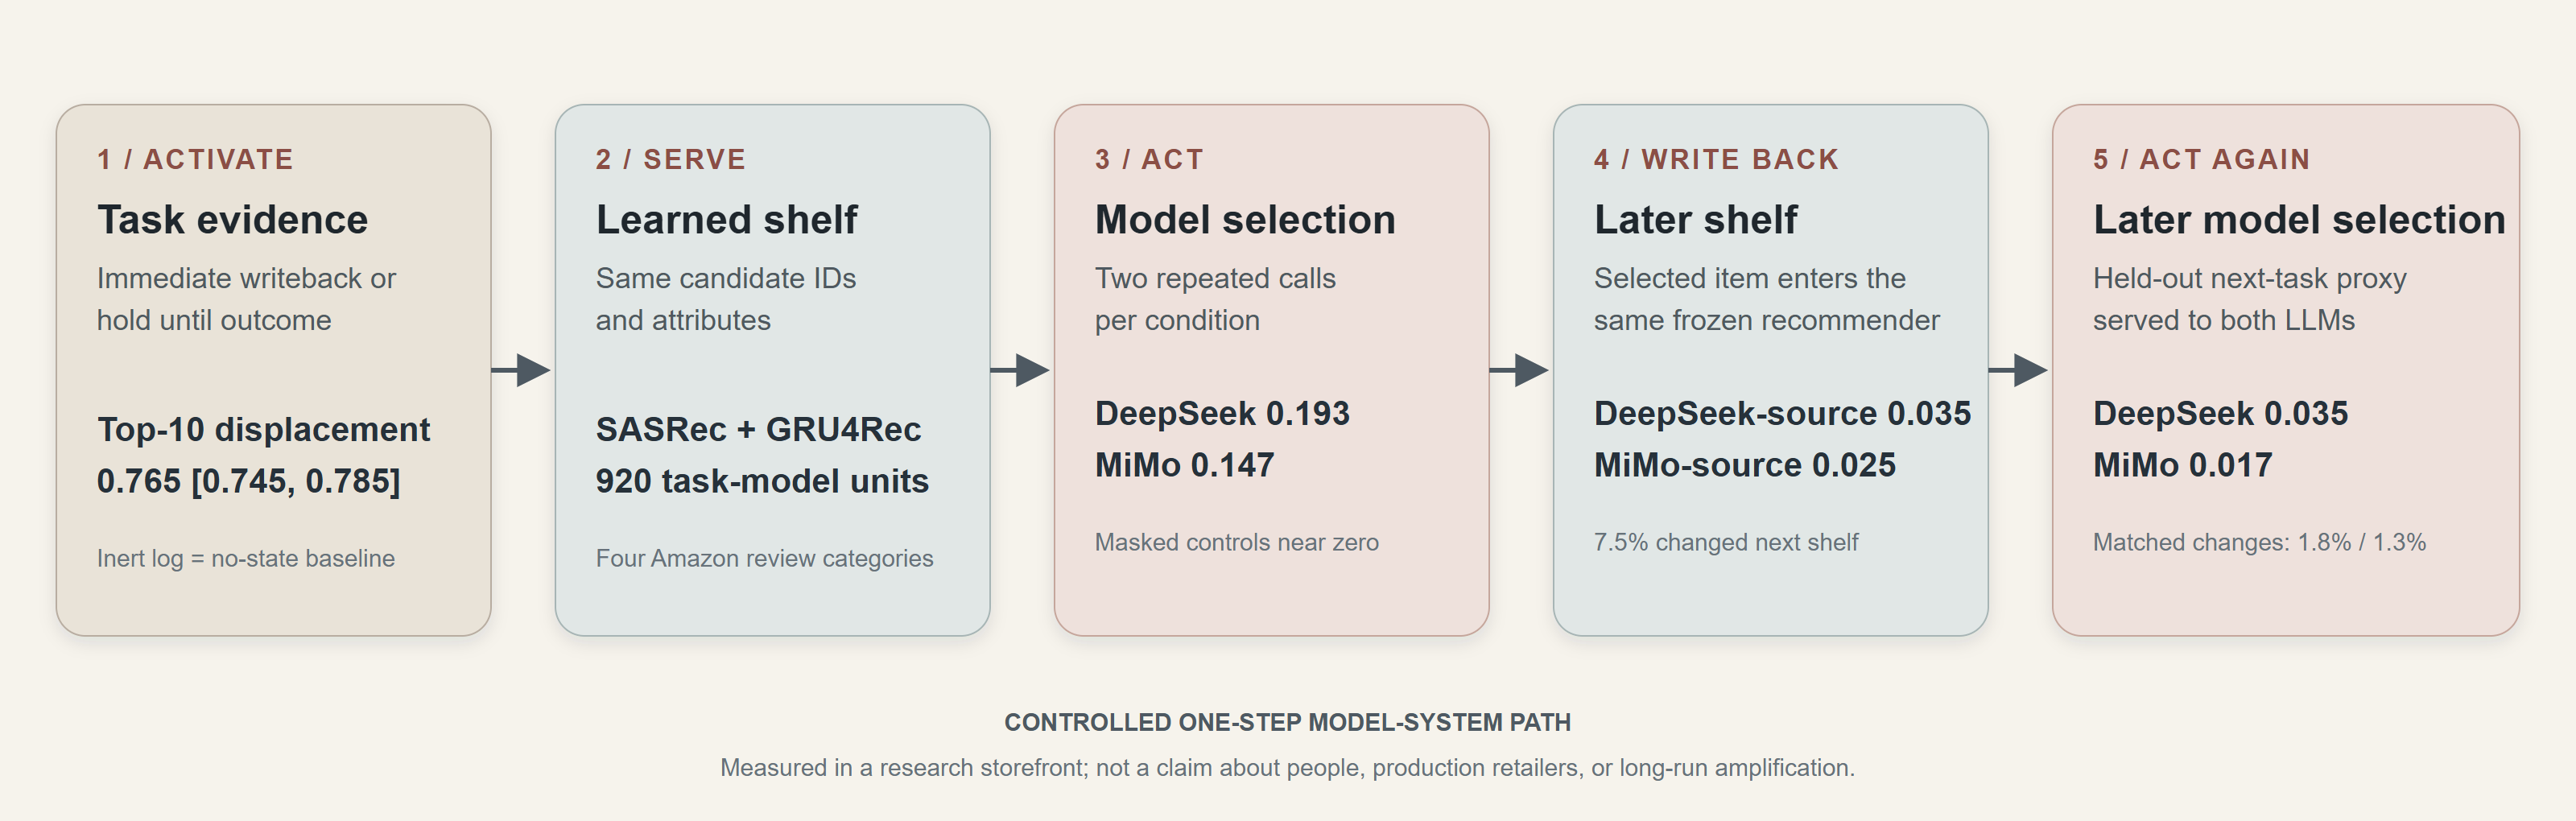
\includegraphics[width=\textwidth]{figures/feedback-chain.png}
  \vspace{-0.9em}
  \caption{Three linked computational studies trace a one-step path. Choice
  distances are mean task-conditional categorical energy U-statistics adjusted
  for within-arm repeat variation.}
  \label{fig:chain}
  \vspace{-0.5em}
\end{figure*}

\section{Research Storefront and Protocols}

We built 460 tasks, 115 per category, from four public Amazon Reviews 2018
sequences \cite{ni2019amazon}. Study 1 used frozen SASRec checkpoints
\cite{kang2018sasrec}. Studies 2 and 3 crossed every task with SASRec and
GRU4Rec \cite{hidasi2016gru4rec}, producing 920 task-model units. During model
calls, the LLMs received pseudonymous IDs and derived scalar features instead
of titles, histories, or review text. DeepSeek V4 Flash and MiMo V2.5 ran at
temperature zero in August 2026. The artifact retains per-call timestamps and
returned model metadata, along with prompt-building code, response schemas,
frozen protocols, and hashed result primitives. It omits provider payloads and
raw responses.

\textbf{Study 1: activation.} We replayed the same behavior and candidate masks
while changing whether temporary task events were logged or activated in the
learned recommender. This comparison isolates recommender activation from event
recording.

\textbf{Study 2: order to action.} For every unit and provider, we used four
input constructions: rank metadata only, inspection state only, a
byte-identical masked control, and served order. The served-order comparison
kept candidate IDs and attributes fixed and changed only their order. Each arm
received two calls, yielding 29,440 valid responses. We used the categorical
energy construction \cite{szekely2013energy}: twice cross-arm disagreement
minus the two within-arm disagreements. Under stable, independent, exchangeable
calls, its mean task-conditional U-statistic estimates squared $L_2$ distance
between categorical output distributions. Two-call unit estimates are noisy
and may be negative. We formed intervals by resampling tasks within category
while retaining both recommender families and every mode. We froze these rules
and the controls before running the study.

\textbf{Study 3: writeback.} We appended each Study 2 selection to the same
frozen recommender history as a standardized positive event. We then added one
held-out next event and generated a new Top-10. The source provider received
this later shelf with a held-out next-task proxy. Each provider retained all
920 units. Within category, recommender, and mode strata,
a frozen four-row cyclic Latin square assigned the four semantic conditions to
call positions; counts differed by at most one. The same 226
protocol-hash-selected units received a byte-identical downstream control.

\textbf{Product-language extension.} In 64 tasks crossed with both recommenders
(128 units; 60 with a feasible offered item), both providers saw
ordinary-language requests and the same 12 cleaned title, brand, and price
records in arm-specific order. We scored task outcomes privately and continued
each trajectory for three fixed steps. The continuation compared selected
events with one deterministic random realization matched on write count and
whether paired writes were equal.

\section{Results}

Logging without activation did nothing. Immediate activation versus holding produced a mean
in-task Top-10 displacement of 0.765 [0.745, 0.785], while no-state and
inert-log shelves agreed. At resolution and the standardized next task, fixed
replay returned to zero displacement.

Order-only exposure changed categorical choices for both providers.
DeepSeek's distance was 0.193 [0.151, 0.239], compared with 0.004 [-0.003,
0.013] in the masked control. MiMo's distance was 0.147 [0.110, 0.187], versus
0.000 [-0.007, 0.008] in its control. All cross-arm changes were swaps between
selectable candidates, not select-to-abandon transitions.

The selected-item difference remained measurable after writeback.
DeepSeek-sourced selections produced later-shelf distance 0.035 [0.024,
0.047]; MiMo-sourced selections produced 0.025 [0.016, 0.035]. Estimates were
positive for SASRec (0.018 [0.010, 0.027]) and GRU4Rec (0.052 [0.034, 0.071]).
Serving later shelves back to their source provider produced distances
0.035 [0.017, 0.054] for DeepSeek and 0.017 [0.005, 0.032] for MiMo; both
226-unit byte-identical controls were zero. Matched repeat-pair change rates were 1.8\%
[1.0\%, 2.8\%] (34/1,840 comparisons; 18/920 units with any change) and 1.3\%
[0.7\%, 2.0\%] (24/1,840; 15/920 units). MiMo's SASRec-only
estimate was 0.007 [-0.004, 0.020], while GRU4Rec was 0.028 [0.009, 0.052].

Across the 128 product-language units, DeepSeek and MiMo order distances were
0.309 [0.180, 0.453] and 0.289 [0.180, 0.414]. Success differences (holding minus immediate)
were 0.031 [-0.008, 0.078] and 0.023 [-0.016, 0.066]; regret and failure also
included zero. At step three, the selected-versus-random difference was 0.007
[-0.023, 0.035] for DeepSeek. For MiMo it was -0.017 [-0.036, -0.001]. Point
estimates did not consistently favor selected writeback, but one random
realization cannot establish equivalence or absence of amplification.

\section{Implications and Limits}

Across the three studies, the initial ordering difference remained measurable
after one writeback cycle in this storefront. We did not compare writeback
policies. Immediate write-then-delete can expose one more shelf to a selection
before deletion, whereas hold-until-outcome would not. Whether that distinction
improves decisions is still unknown. Prior systems separate intent-specific
profiles \cite{tsukuda2025intent}, recommendation memories
\cite{zhan2026calmrec}, memory admission \cite{xiong2026memory}, or agents from
platforms \cite{xu2025iagent}. Our study instead estimates how much an order
effect attenuates after the selected item mediates writeback. A future interface
could keep task-local assistance while delaying admission to the account
history, but this study does not test that interface.

There are no human participants; the counterfactual tasks are not observed
delegations. The final endpoint uses pseudonymous scalars and a held-out-item
proxy. The 64-task extension uses cleaned metadata, but its token-and-price
score is not human utility; later steps use a fixed policy instead of repeated
LLM calls. Two repeats per arm limit stationarity assessment. DeepSeek returned
one provider fingerprint, while MiMo returned none, and the order-specific
estimates were imprecise. The single random-writeback realization is not an
equivalence test. The one-step
horizon and matched endpoint rates between 1.3\% and 1.8\% do not establish harm
or amplification.
Future work should ask whether people want actor provenance and task outcome to
govern account-history admission.

\paragraph{Generative AI disclosure.} Generative AI tools assisted with code
generation, experiment orchestration, and language editing. The author checked
the protocols, statistical decisions, sources, and reported results against the
frozen artifacts included with the submission.

\balance
\bibliographystyle{ACM-Reference-Format}
\bibliography{references}

\end{document}
